\documentclass[conference]{IEEEtran}

\usepackage[T1]{fontenc}
\usepackage{mathptmx}
\usepackage{graphicx}
\usepackage{booktabs}
\usepackage{amsmath}
\usepackage{multirow}
\usepackage[hidelinks]{hyperref}
\usepackage{url}

\graphicspath{{../figures/}}

% ---------------------------------------------------------------------------
% ANONYMIZED SUBMISSION (IEEE CogMI 2026 requires anonymized review copies).
% For the camera-ready, comment the anonymous block and uncomment the named
% block below.
% ---------------------------------------------------------------------------

\begin{document}

\title{Cheap to Verify, Expensive to Fix: Deterministic Structural
Verification as a Routing Signal for Matched-Cost VLM Table Extraction}

\author{\IEEEauthorblockN{Anonymous submission}}
% CAMERA-READY (de-anonymize on acceptance):
% \author{\IEEEauthorblockN{Michael Hamaty}%
% \IEEEauthorblockA{San Jose State University, San Jose, CA, USA}}

\maketitle

\begin{abstract}
\normalfont
Vision-language models (VLMs) used for table extraction spend the same
visual tile budget on every page, regardless of difficulty. We study a
simple alternative: parse each page once at a low tile budget, check the
emitted HTML with a deterministic structural verifier (parseability, span
consistency, grid rectangularity, table presence), and reparse the page
once at a higher budget only if the check fails. The verifier requires no
training, no OCR, and no reference output, and each routing decision can
be audited by re-running a parser. We evaluate this policy under a
matched-cost protocol in which the adaptive system, a fixed-budget
baseline, and a random-escalation control matched in expected cost all
spend a near-equal mean tile budget per page, with budgets frozen on
separate calibration splits. On held-out FinTabNet pages (n=150,
InternVL2-2B), verifier-gated escalation reaches 0.133 macro cell-F1
versus 0.120 for the cost-matched fixed baseline, and its advantage over
random escalation at equal expected cost is the only contrast that remains
significant after Holm correction (paired Wilcoxon, adjusted
p\,$=$\,0.0007). The gain persists against a post-hoc 11-tile baseline
given more budget than the adaptive system, although the fixed-baseline
contrast itself stays borderline (p\,$\approx$\,0.05--0.06). On held-out
OmniDocBench pages (n=90) the policy shows no measurable gain: escalation
becomes nearly uniform (78\% of pages) and adaptive, random, and fixed
systems are statistically indistinguishable. The contrast suggests that
structural verification is a useful routing signal precisely where uniform
budget increases have weak returns, and adds little where most pages need
the higher budget anyway. We report verifier failure-code distributions,
per-page reparse outcomes, and wall-clock measurements showing that
matched tile budgets do not imply matched latency.
\end{abstract}

\begin{IEEEkeywords}
vision-language models, adaptive inference, table extraction, structural
verification, matched-cost evaluation, document understanding
\end{IEEEkeywords}

% ===========================================================================
\section{Introduction}
\label{sec:intro}
% ===========================================================================

A VLM-based table extractor commits the same per-page compute whether the
page holds a short list as opposed to a dense financial statement with merged
cells. Modern open VLMs such as InternVL2 expose this compute as a visual
tile budget: the page image is split into up to $B$ fixed-resolution tiles
before encoding, so the budget is an explicit, per-request
knob~\cite{chen2024internvl,chen2024internvl15}. Fixed-budget inference
spends most of that budget on pages that did not need it.

Table extraction has a property that makes a cheap routing signal
plausible: the output format has crisp syntactic invariants. A predicted
HTML table either parses or it does not; its
\texttt{rowspan}/\texttt{colspan} declarations either expand into a
rectangular cell grid or they do not; a page either contains a
\texttt{<table>} element or it does not. Checking these invariants takes
under two milliseconds per page in our measurements, while a single 2B
model pass takes tens of seconds on the same hardware: verification is
cheap; producing a better parse is expensive.

This paper addresses a specific question: can a deterministic structural
check on the model's own output route a second, higher-budget parse to
the pages that need it, well enough to beat spending the same average
tile budget uniformly, and more stringently, to beat spending it
randomly? The random-escalation control matters as much as the fixed
baseline. Any escalation policy buys extra compute for some pages; if
random escalation at the same probability does as well as the
verifier, the verifier signal carries no information. Our protocol
therefore compares the adaptive system against fixed-budget baselines
\emph{and} a random control matched in expected tile cost, with all
budgets frozen on calibration data before the held-out evaluation.

We make three contributions.
\begin{enumerate}
  \item \textbf{An auditable, training-free routing mechanism.} A
  deterministic verifier over emitted table HTML (five failure codes;
  Section~\ref{sec:verifier}) gates a single full-page reparse at a higher
  tile budget. There is no learned router, no OCR on the trigger path,
  and at most one reparse per page; every routing decision can be
  reproduced from the page's raw output alone.
  \item \textbf{A matched-cost evaluation protocol with a random
  control.} Budgets are calibrated and frozen on separate 50-page splits
  per dataset; the held-out comparison includes a low-budget floor, a
  cost-matched fixed baseline, a random-escalation control at the
  calibration-measured escalation rate (three seeds), a tile-matched 8B
  reference, and a post-hoc over-budget fixed baseline that brackets the
  adaptive system's realized cost from above. Paired tests are reported
  with Holm correction across the confirmatory family.
  \item \textbf{A conditional empirical result on two datasets.} On
  FinTabNet (150 held-out pages) the verifier-gated policy beats random
  escalation at equal expected cost (the only Holm-significant contrast)
  and shows a consistent $+0.014$ cell-F1 margin over fixed baselines at
  both 10 and 11 tiles. On OmniDocBench (90 held-out pages) the policy
  shows no gain over either control. The budget-response curves of the
  two datasets explain the split: uniform budget increases barely help
  FinTabNet but help OmniDocBench a great deal, leaving selective
  escalation no room to win there.
\end{enumerate}

We also report what fixed-budget evaluations usually omit: verifier
failure-code distributions, per-page reparse outcomes (improved,
unchanged, regressed), per-seed random-control variance, and wall-clock
latency, which shows that matching tile budgets does not match latency.

% ===========================================================================
\section{Related Work}
\label{sec:related}
% ===========================================================================

\textbf{VLM document and table parsing.} End-to-end vision-language
models have largely replaced detect-then-recognize cascades for document
parsing. Donut~\cite{kim2022donut} and Pix2Struct~\cite{lee2023pix2struct}
treat parsing as conditional generation from pixels; open VLM families
such as InternVL~\cite{chen2024internvl} provide size-paired checkpoints
(2B/8B)~\cite{opengvlab2024internvl2} and a dynamic tiling mechanism~\cite{chen2024internvl15} that
makes visual compute an explicit budget. Table-structure work, including
TableFormer~\cite{nassar2022tableformer} and
PubTables-1M~\cite{smock2022pubtables}, together with the PubTabNet
benchmark and its TEDS metric~\cite{zhong2020teds},
TableBank~\cite{li2020tablebank}, and
FinTabNet~\cite{zheng2021fintabnet}, established the datasets and metrics
we build on. Throughout this line of work, inference is fixed-budget: no
mechanism decides per page where extra visual budget should go.

\textbf{Adaptive computation.} Spending more compute on harder inputs has
a long history, from cascaded detectors~\cite{viola2001rapid} and
early-exit networks~\cite{teerapittayanon2016branchynet} to adaptive
computation time~\cite{graves2016act}, confidence-based early exit in
language models~\cite{schuster2022calm}, speculative
decoding~\cite{leviathan2023speculative}, and cost-aware model
cascades~\cite{chen2023frugalgpt}. These mechanisms typically rely on a
\emph{learned} signal, such as a halting unit, a confidence head, or a trained
router. Our escalation signal is instead a deterministic predicate on the
structured output itself, which removes training-data requirements and
makes individual routing decisions inspectable.

\textbf{Output verification and self-correction.} Verifier-guided
generation usually employs a learned critic: trained solution verifiers
for math~\cite{cobbe2021verifiers}, process supervision
~\cite{lightman2024verify}, model self-critique~\cite{madaan2023selfrefine},
or agreement-based selection over samples~\cite{wang2023selfconsistency}.
A learned critic can judge content but is itself a model with failure
modes and training costs. We restrict the checker to structural
well-formedness; it can only declare an output structurally acceptable
or not, and it cannot rewrite anything. This narrow contract is what
makes the check deterministic, near-zero-cost, and auditable.

The gap this paper addresses sits at the intersection: fixed-budget VLM
table extraction does not allocate visual budget per page; adaptive
computation methods allocate but need learned signals; verification work
supplies signals but usually learned ones. We evaluate the simplest
such signal, a deterministic structural predicate used as
the routing signal, under matched-cost controls designed to detect
whether the signal itself, rather than the extra compute, produces any
gain.

% ===========================================================================
\section{Verifier-Gated Adaptive Inference}
\label{sec:system}
% ===========================================================================

\begin{figure*}[t]
  \centering
  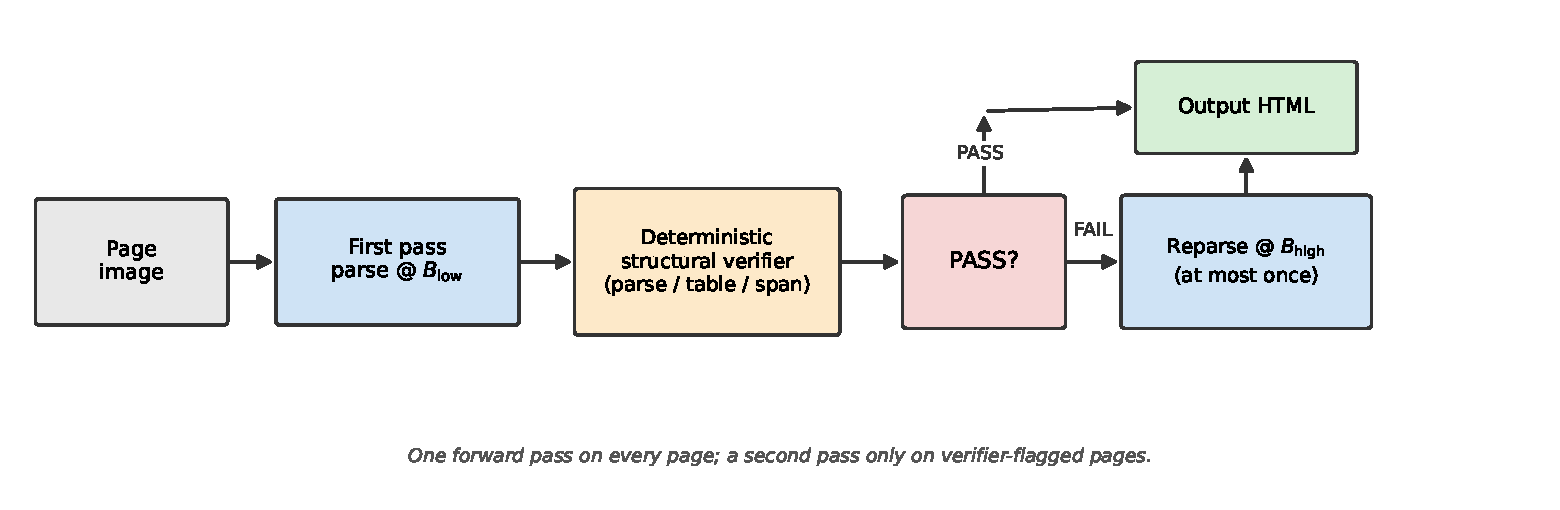
\includegraphics[width=0.92\textwidth]{system_overview.pdf}
  \caption{The adaptive pipeline. Every page is parsed once at the low
  tile budget $B_{\mathrm{low}}$. A deterministic structural verifier
  inspects the emitted HTML and either accepts the first pass or triggers
  exactly one reparse at $B_{\mathrm{high}}$, whose output then replaces
  the first pass. There is no learned routing, no OCR, and no second
  reparse.}
  \label{fig:overview}
\end{figure*}

Figure~\ref{fig:overview} shows the pipeline. We describe the backbone
and prompt, the verifier, the escalation policy, and the cost model that
the matched-cost protocol relies on.

\subsection{Setting and backbone}
\label{sec:setting}

We use InternVL2-2B for all 2B systems and InternVL2-8B for the 8B
reference, loaded from the public checkpoints~\cite{opengvlab2024internvl2} with bfloat16 weights on a
single NVIDIA L4 (24\,GB). InternVL2 splits each page image into at most
$B$ fixed-resolution tiles before visual encoding, so $B$ (``max tiles'')
upper-bounds visual compute per pass; under a fixed prompt and greedy
decoding it is the only per-request compute knob we vary. All systems
share one fixed prompt that instructs the model to transcribe the page
and emit every table as raw HTML \texttt{<table>} markup, explicitly
forbidding markdown pipe tables and bulleted reformatting; decoding is
greedy with a 2{,}048-token cap, no sampling anywhere. Because decoding
is greedy, the adaptive system's first pass is bit-for-bit the
low-budget baseline: across all 240 held-out pages the two produced
identical output token counts.

One implementation detail affects runtime and is disclosed for
reproducibility. On hard pages the 2B model sometimes degenerates into an
exactly periodic token loop and runs to the 2{,}048-token cap. The
adapter detects exact periodicity over a trailing 100-token window
(period $\le$ 50) and truncates the repeating tail. The detector never
alters which tokens are chosen; it only stops obvious loops early.
Re-running the frozen calibration points under it left tile budgets
unchanged (one borderline FinTabNet page changed its reparse decision,
shifting measured adaptive cost from 10.16 to 10.48 tiles per page; the
frozen artifact records the re-measured value, and the random control's
escalation probability is derived from it).

\subsection{Deterministic structural verifier}
\label{sec:verifier}

The verifier is a pure function from the raw output string to a decision
in \{\textsc{pass}, \textsc{reparse}\} plus a set of failure codes. It
extracts \texttt{<table>} blocks from the output, then for each block
attempts HTML parsing, expands \texttt{rowspan}/\texttt{colspan}
declarations into a flat cell grid, and checks the grid. Five failure
codes exist:

\begin{itemize}
  \item \texttt{NO\_TABLE\_FOUND}, the output contains no
  \texttt{<table>} block;
  \item \texttt{HTML\_PARSE\_ERROR}, a block exists but does not parse;
  \item \texttt{SPAN\_EXPANSION\_FAILED}, span attributes cannot be
  resolved into a grid;
  \item \texttt{RECTANGULAR\_INCONSISTENCY}, after span expansion, row
  lengths disagree;
  \item \texttt{DEGENERATE\_TABLE}, the grid is empty or all cells are
  blank.
\end{itemize}

Any failure code on any block yields \textsc{reparse}. The verifier
consults no reference output, no model, and no OCR; it performs no
semantic checks, so a well-formed table with wrong content passes. It is
intentionally a high-precision trigger for \emph{structural} breakage,
not a correctness oracle. Measured on the held-out runs, verification
costs at most 1.6\,ms per page (median 0.04--0.39\,ms), against a mean of
17--33\,s per model pass on the same machine: negligible relative to
inference, though not literally free.

\subsection{Escalation policy}
\label{sec:policy}

The policy is one rule: if the verifier returns \textsc{reparse}, run the
same model on the same full page once more at $B_{\mathrm{high}}$, and
keep the second output unconditionally; otherwise keep the first. At most
one reparse per page is permitted, enforced structurally by the runner.
We deliberately add no heuristics on top: no output-length checks, no
retry on the second pass, and no selection between the two outputs. Keeping
the replacement unconditional means a reparse \emph{can} in principle
produce a worse parse than the first pass; whether that happens is an
empirical question we report on in Section~\ref{sec:diagnostics}.

\subsection{Cost model}
\label{sec:cost}

Our pre-registered cost unit is the per-page tile budget. A fixed system
at budget $B$ costs $B$ tiles per page. The adaptive system costs
\begin{equation}
  c_i \;=\; B_{\mathrm{low}} + r_i\, B_{\mathrm{high}},
  \qquad r_i \in \{0,1\},
  \label{eq:cost}
\end{equation}
where $r_i$ indicates a reparse on page $i$; the mean cost over a split
is $B_{\mathrm{low}} + \bar{p}\,B_{\mathrm{high}}$ with $\bar{p}$ the
empirical reparse rate. Tile budget is the right \emph{control} variable;
it is the knob the systems actually differ on, it is deterministic,
and visual-encoder compute scales with it; but it is not wall-clock
latency and it is not FLOPs. Two passes carry fixed overheads, decode
length varies, and an 8B model at the same tile count performs roughly
four times the work per token of a 2B model. We therefore match systems
on tiles, state so explicitly, and report measured wall-clock alongside
(Section~\ref{sec:runtime}); we avoid the phrase ``equal compute.''

% ===========================================================================
\section{Experimental Design}
\label{sec:design}
% ===========================================================================

\subsection{Datasets, filtering, and splits}
\label{sec:datasets}

We evaluate on English table pages from two sources with deliberately
different character.

\textbf{OmniDocBench}~\cite{ouyang2024omnidocbench} provides
diverse-source PDF pages with gold HTML table annotations. We keep pages
annotated as English with at least one table whose gold cells include at
least four non-empty entries. The filter exists because the source
occasionally tags layout scaffolding (slide bullet groups, mostly-empty
forms) as tables; such pages score near zero for every system regardless
of quality and only add noise. The filtered English-table population is
146 pages; we use 140: 50 for calibration and 90 held out.

\textbf{FinTabNet}, introduced as part of the GTE framework~\cite{zheng2021fintabnet}, contains financial-report
pages with dense, span-heavy tables. We draw from the HTML-paired
distribution of its test split, cap at 250 candidate pages, apply the
same four-cell filter, and stratify-sample 200 pages by a difficulty
bucketing (below): 50 for calibration, 150 held out.

Difficulty buckets are computed from gold metadata: \emph{simple} (fewer
than 6 rows), \emph{complex} (6--15 rows), \emph{very complex} (16+ rows
or any merged cell). The held-out splits skew hard: 51 of 90 OmniDocBench
pages and 91 of 150 FinTabNet pages are very complex. Calibration and
held-out splits are disjoint; budgets were never re-selected on held-out
pages.

\subsection{Budget calibration}
\label{sec:calibration}

For each dataset independently, a sweep on the 50-page calibration split
selects the budget pair $(B_{\mathrm{low}}, B_{\mathrm{high}})$ whose
measured mean adaptive cost (Eq.~\ref{eq:cost}) lies closest to a target
of 10 tiles per page, then freezes the matched fixed budgets at the
nearest integer to the measured adaptive cost. The frozen values are
shown in Table~\ref{tab:budgets}. Because fixed budgets live on an
integer grid, exact equality with the adaptive system's realized cost is
not attainable; on FinTabNet we therefore additionally evaluate a
post-hoc 11-tile fixed baseline that brackets the adaptive system's
held-out cost (10.37 tiles) from above
(Section~\ref{sec:overmatch}).

\begin{table}[t]
  \centering
  \caption{Frozen per-dataset budgets (max tiles) and
  calibration-measured quantities. The random control's per-page
  escalation probability $\hat{p}$ is derived from the frozen artifact as
  $(\bar{c}_{\mathrm{cal}} - B_{\mathrm{low}})/B_{\mathrm{high}}$.}
  \label{tab:budgets}
  \footnotesize
  \setlength{\tabcolsep}{4pt}
  \begin{tabular}{lcc}
  \toprule
   & OmniDoc. & FinTab. \\
  \midrule
  $B_{\mathrm{low}}$ / $B_{\mathrm{high}}$ & 2 / 12 & 6 / 16 \\
  $B^{\mathrm{fix}}$ (2B and 8B)           & 11     & 10 \\
  Measured adaptive cost $\bar{c}_{\mathrm{cal}}$ & 10.64 & 10.48 \\
  Reparse rate                             & 0.72   & 0.28 \\
  Random control $\hat{p}$                 & 0.72   & 0.28 \\
  \bottomrule
  \end{tabular}
\end{table}

\subsection{Systems}
\label{sec:systems}

Seven runs per dataset, identical prompt, weights per model size,
decoding, page order, and scorer:

\begin{itemize}
  \item \texttt{fixed\_2b\_low}: single pass at $B_{\mathrm{low}}$. The
  floor, and (by greedy determinism) identical to the adaptive system's
  first pass.
  \item \texttt{fixed\_2b\_matched}: single pass at $B^{\mathrm{fix}}$,
  the uniform-spending competitor at matched mean tile cost.
  \item \texttt{adaptive\_2b}: the pipeline of Section~\ref{sec:system}.
  \item \texttt{random\_2b\_seed\{0,1,2\}}: identical two-pass shape, but
  the verifier decision is discarded and replaced by an independent
  Bernoulli($\hat{p}$) draw with $\hat{p}$ from
  Table~\ref{tab:budgets}. This control separates the value of the
  \emph{signal} from the value of the \emph{extra compute}: if the
  verifier carries no information, adaptive and random should perform
  alike at equal expected cost.
  \item \texttt{fixed\_8b\_matched}: InternVL2-8B, single pass at
  $B^{\mathrm{fix}}$. A reference for ``spend the budget on a bigger
  model'', matched in tiles, not in FLOPs (Section~\ref{sec:cost}).
\end{itemize}

\subsection{Metrics}
\label{sec:metrics}

\textbf{Macro cell-F1} (primary). Predicted and gold HTML are parsed with
the same span expander the verifier uses; each cell becomes a tuple
(table index, row, column, whitespace-normalized text), and per-page F1
is computed over exact tuple matches, then averaged unweighted across
pages. Pages whose predicted HTML fails parsing or grid expansion score
zero; malformed output is penalized, not repaired. The metric is
strict: a table that is shifted by one column scores near zero even if
its text is right.

\textbf{TEDS} (secondary)~\cite{zhong2020teds}: tree-edit-distance
similarity over the parsed table trees, following the reference
implementation's structure. TEDS gives partial credit where cell-F1 does
not, so reporting both bounds the metric sensitivity of our conclusions.

\textbf{Parse-error count}: pages whose prediction failed HTML parsing or
span expansion outright.

All means carry 95\% bootstrap confidence intervals (percentile, $10^4$
resamples).

\subsection{Statistical protocol}
\label{sec:stats}

We pre-specify four confirmatory paired comparisons on per-page cell-F1,
namely \{adaptive vs.\ fixed-matched, adaptive vs.\ random\} $\times$
\{OmniDocBench, FinTabNet\}, tested with two-sided Wilcoxon
signed-rank tests and Holm correction across the family of four. For the
random control, the three seeds are pooled by averaging each page's
cell-F1 across seeds before pairing, so each page contributes one pair
(no pseudo-replication); per-seed means and their spread are reported
separately. Pairs with zero difference are dropped, per the standard
zero-method; because many hard pages score zero under every system, the
number of informative (non-tied) pairs is small, and we report it for
every test. The post-hoc 11-tile comparison is labeled exploratory and is
not part of the corrected family; for it we also report a bootstrap CI on
the mean paired difference.

% ===========================================================================
\section{Results}
\label{sec:results}
% ===========================================================================

\subsection{Main matched-cost comparison}
\label{sec:main}

Table~\ref{tab:main} reports all systems on both held-out splits;
Figure~\ref{fig:budget} plots the same data against tile budget. Realized
mean tile costs confirm the protocol: on OmniDocBench the adaptive system
spent 11.33 tiles per page against the fixed baseline's 11.0, and on
FinTabNet 10.37 against 10.0. The adaptive system was, if anything,
slightly over-budgeted, which makes its OmniDocBench null result
conservative and motivates the over-budget check of
Section~\ref{sec:overmatch} for FinTabNet.

\begin{table*}[t]
  \centering
  \caption{Held-out results. Cost is mean visual tiles per page
  (realized, from Eq.~\ref{eq:cost} for two-pass systems). Cell-F1 and
  TEDS are macro means with 95\% bootstrap CIs; parse-err counts pages
  whose prediction failed parsing or grid expansion. The random rows
  show each seed, since the three seeds are separate runs. The 11-tile
  FinTabNet baseline is the post-hoc over-budget check of
  Section~\ref{sec:overmatch}.}
  \label{tab:main}
  \small
  \begin{tabular}{llrllr}
  \toprule
  Dataset & System & Cost & Macro cell-F1 [95\% CI] & TEDS [95\% CI] & Parse-err \\
  \midrule
  \multirow{7}{*}{\shortstack[l]{OmniDocBench\\(n=90)}}
   & fixed 2B low (2 tiles)      &  2.00 & 0.039 [0.010, 0.075] & 0.106 [0.067, 0.152] & 70 \\
   & fixed 2B matched (11 tiles) & 11.00 & 0.120 [0.070, 0.173] & 0.268 [0.214, 0.325] & 57 \\
   & adaptive 2B                 & 11.33 & 0.121 [0.071, 0.175] & 0.274 [0.214, 0.333] & 45 \\
   & random 2B seed 0            & 11.20 & 0.123 [0.074, 0.179] & 0.249 [0.195, 0.310] & 55 \\
   & random 2B seed 1            & 11.47 & 0.120 [0.069, 0.172] & 0.245 [0.186, 0.300] & 51 \\
   & random 2B seed 2            & 10.13 & 0.100 [0.055, 0.149] & 0.221 [0.163, 0.280] & 61 \\
   & fixed 8B matched (11 tiles) & 11.00 & 0.200 [0.132, 0.271] & 0.396 [0.326, 0.469] & 38 \\
  \midrule
  \multirow{8}{*}{\shortstack[l]{FinTabNet\\(n=150)}}
   & fixed 2B low (6 tiles)      &  6.00 & 0.130 [0.089, 0.174] & 0.483 [0.435, 0.527] & 41 \\
   & fixed 2B matched (10 tiles) & 10.00 & 0.120 [0.078, 0.164] & 0.465 [0.416, 0.508] & 37 \\
   & fixed 2B over-budget (11 tiles) & 11.00 & 0.120 [0.078, 0.164] & 0.462 [0.414, 0.506] & 37 \\
   & adaptive 2B                 & 10.37 & 0.133 [0.092, 0.179] & 0.492 [0.447, 0.535] & 30 \\
   & random 2B seed 0            &  9.95 & 0.116 [0.075, 0.159] & 0.462 [0.417, 0.506] & 41 \\
   & random 2B seed 1            &  9.84 & 0.119 [0.080, 0.162] & 0.476 [0.430, 0.519] & 44 \\
   & random 2B seed 2            & 11.55 & 0.124 [0.085, 0.169] & 0.472 [0.426, 0.517] & 42 \\
   & fixed 8B matched (10 tiles) & 10.00 & 0.134 [0.092, 0.182] & 0.527 [0.481, 0.573] & 46 \\
  \bottomrule
  \end{tabular}
\end{table*}

\begin{figure*}[t]
  \centering
  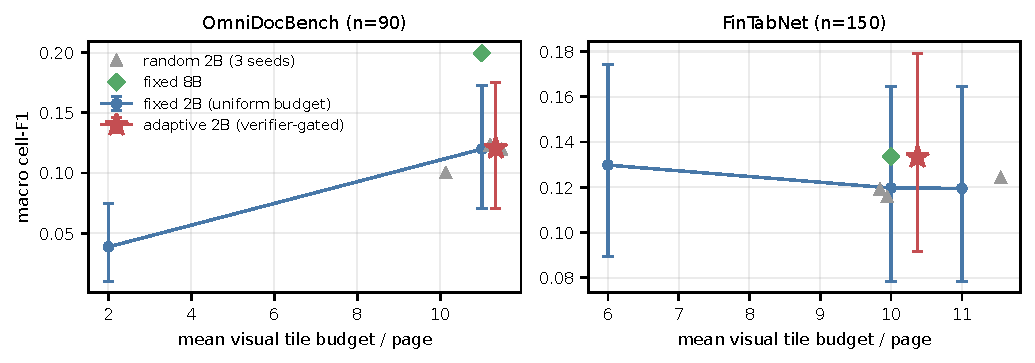
\includegraphics[width=0.94\textwidth]{budget_response.pdf}
  \caption{Macro cell-F1 against mean tile budget (bars: 95\% bootstrap
  CIs). The two datasets respond to uniform budget in opposite ways.
  OmniDocBench (left) rises steeply from 2 to 11 tiles, and the adaptive
  policy lands on the fixed-budget line: selective escalation has nothing
  to add when uniform spending already pays. FinTabNet (right) is flat to
  slightly negative from 6 to 11 tiles; more uniform budget does not
  help. Yet the verifier-gated system sits above every same-cost 2B
  alternative and at the level of the tile-matched 8B reference.}
  \label{fig:budget}
\end{figure*}

Three observations are relevant to the results that follow. First, on FinTabNet,
uniform budget increases do not help: the 6-tile floor (0.130) already
exceeds the 10-tile (0.120) and 11-tile (0.120) fixed systems. Second, on
OmniDocBench the opposite holds; cell-F1 triples from 2 to 11 tiles
(0.039 to 0.120), and only the 8B model (0.200) rises above the 2B
cluster. Third, the adaptive system is the best 2B system on FinTabNet
(0.133) while reducing parse errors on both datasets (45 vs.\ 57 on
OmniDocBench, 30 vs.\ 37 on FinTabNet relative to fixed-matched).

\subsection{Does the verifier signal beat its controls?}
\label{sec:tests}

\begin{table}[t]
  \centering
  \caption{Paired Wilcoxon tests on per-page cell-F1. The first four rows
  are the pre-specified confirmatory family (Holm-corrected); the last
  row is the post-hoc over-budget check (exploratory, uncorrected, with a
  bootstrap CI on the mean paired difference). ``Inf.\ pairs'' counts
  non-tied pairs actually entering each test; ties at zero are common
  because many very-complex pages score 0 under every system.}
  \label{tab:tests}
  \footnotesize
  \setlength{\tabcolsep}{2.5pt}
  \resizebox{\columnwidth}{!}{%
  \begin{tabular}{llrrrr}
  \toprule
  Dataset & Comparison & $\Delta$ & Inf.\ pairs & $p$ & $p_{\mathrm{Holm}}$ \\
  \midrule
  FinTab  & adapt.\ vs.\ random   & $+0.0138$ & 29/150 & $1.8{\times}10^{-4}$ & $\mathbf{7.0{\times}10^{-4}}$ \\
  FinTab  & adapt.\ vs.\ fixed 10 & $+0.0137$ & 13/150 & 0.048 & 0.144 \\
  OmniDoc & adapt.\ vs.\ random   & $+0.0066$ & 26/90  & 0.269 & 0.538 \\
  OmniDoc & adapt.\ vs.\ fixed 11 & $+0.0009$ & 32/90  & 0.729 & 0.729 \\
  \midrule
  FinTab  & adapt.\ vs.\ fixed 11 & $+0.0139$ & 51/150 & 0.058 & --- \\
  \multicolumn{6}{l}{\quad bootstrap 95\% CI of mean difference: $[+0.002,\, +0.029]$} \\
  \bottomrule
  \end{tabular}}
\end{table}

Table~\ref{tab:tests} reports the confirmatory paired comparisons. One
contrast survives Holm correction: on FinTabNet, the adaptive system
beats the pooled random-escalation control by $+0.0138$ cell-F1 at equal
expected tile cost (adjusted $p = 7.0\times10^{-4}$). Random escalation
at the same rate does not reproduce the adaptive gain; per-seed means are
0.116, 0.119, 0.124 (s.d.\ 0.004) against the adaptive 0.133, so on
this dataset the verifier's choice of \emph{which} pages to escalate
carries measurable information beyond the escalation budget itself.

The FinTabNet adaptive-versus-fixed-matched contrast does not survive
correction ($p = 0.048$ raw, $0.144$ adjusted) and we do not claim it as
significant. Its effect size, however, is consistent: $+0.0137$ against
the 10-tile baseline and $+0.0139$ against the post-hoc 11-tile baseline,
with a bootstrap CI on the latter difference excluding zero. With 137 of
150 pairs tied (mostly pages scoring zero under both systems), the rank
test is powered by 13 informative pages; the borderline p-values reflect
that, and a larger evaluation would be needed to settle the
fixed-baseline contrast either way.

On OmniDocBench both confirmatory contrasts are null ($p \ge 0.27$ raw).
Adaptive, random, and fixed-matched are statistically indistinguishable
there, and we treat this as a finding rather than a failure: the policy
escalated 70 of 90 pages (78\%), so it nearly reproduces uniform
high-budget spending, and no escalation rule that fires on almost every
page can beat either uniform or random spending at the same rate.

\subsection{The over-budget check}
\label{sec:overmatch}

Because the adaptive system's realized FinTabNet cost (10.37 tiles)
exceeds the frozen fixed baseline (10.0), its margin could be attributed
to the extra 0.37 tiles rather than to routing. After the held-out
results were known, we ran one additional fixed baseline at 11 tiles,
\emph{more} budget than the adaptive system used, under the identical
prompt, weights, decoding, and scorer, and we report it regardless of
outcome. The extra tile bought nothing: 0.1195 cell-F1 versus 0.1197 at
10 tiles, with parse errors unchanged (37). The adaptive margin persists
($+0.0139$, CI $[+0.002, +0.029]$), bracketing the adaptive cost from
both sides: spending \emph{less} than adaptive (10 tiles), the same
uniform policy scores 0.120; spending \emph{more} (11 tiles), 0.120;
routing the same average budget with the verifier, 0.133. We label this
comparison exploratory; it was chosen post hoc, and its rank-test
p-value (0.058) is as borderline as the 10-tile one. But it removes
the budget-mismatch explanation for the FinTabNet effect: on this
dataset the gain tracks \emph{where} tiles were spent, not how many.

\subsection{Verifier diagnostics}
\label{sec:diagnostics}

\begin{table}[t]
  \centering
  \caption{Verifier behavior on held-out first passes, and the outcome of
  every triggered reparse on per-page cell-F1. Outcomes are observations,
  not guarantees: the reparse output replaces the first pass
  unconditionally.}
  \label{tab:verifier}
  \footnotesize
  \setlength{\tabcolsep}{3.5pt}
  \begin{tabular}{lrr}
  \toprule
   & OmniDoc. & FinTab. \\
  \midrule
  Pages (held-out)                   & 90 & 150 \\
  Reparse triggered                  & 70 (78\%) & 41 (27\%) \\
  \quad {\scriptsize\texttt{NO\_TABLE\_FOUND}}    & 69 & 28 \\
  \quad {\scriptsize\texttt{RECTANGULAR\_INCONSISTENCY}} & 1 & 13 \\
  \quad other three codes            & 0 & 0 \\
  \midrule
  Reparse improved cell-F1           & 20 & 6 \\
  Reparse left cell-F1 unchanged     & 50 & 35 \\
  Reparse lowered cell-F1            & 0 & 0 \\
  \bottomrule
  \end{tabular}
\end{table}

\begin{figure}[t]
  \centering
  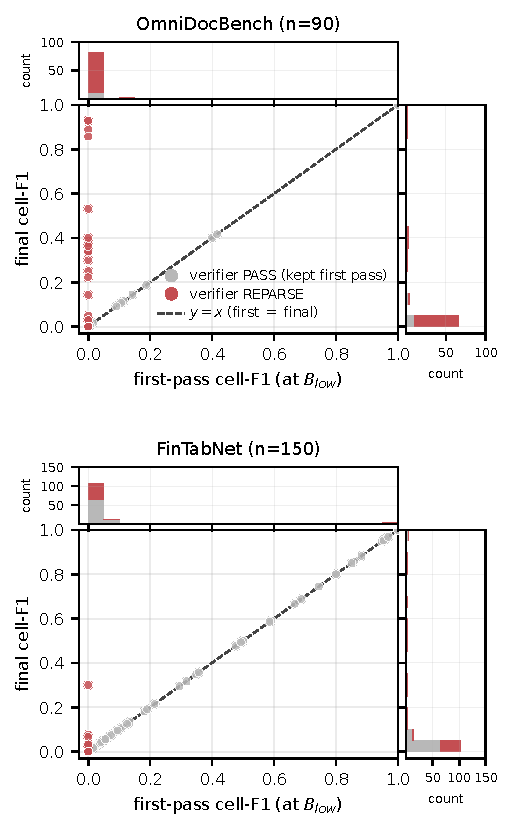
\includegraphics[width=0.96\linewidth]{adaptive_scatter.pdf}
  \caption{Per-page first-pass vs.\ final cell-F1 for the adaptive
  system, colored by the verifier's actual decision. Gray
  (\textsc{pass}) pages lie on the diagonal by construction; the first
  pass is kept. Red (\textsc{reparse}) pages above the diagonal gained
  from the second pass; most OmniDocBench gains start from a first-pass
  score of zero, consistent with the \texttt{NO\_TABLE\_FOUND}-dominated
  trigger profile. No page fell below the diagonal in these runs.}
  \label{fig:scatter}
\end{figure}

Table~\ref{tab:verifier} and Figure~\ref{fig:scatter} open the routing
decisions to inspection. Two of the five failure codes fired on held-out
data. The trigger profile differs by dataset in an interpretable way:
OmniDocBench failures are almost entirely missing tables (69 of 70);
at 2 tiles the model often transcribes the page without emitting
\texttt{<table>} markup at all. FinTabNet, whose first pass
already runs at 6 tiles, instead mixes missing tables (28) with span-expansion
inconsistencies (13), consistent with partially malformed complex tables.

The reparse yield is modest. On OmniDocBench,
20 of 70 reparses improved the page's cell-F1; on FinTabNet, 6 of 41. The
remaining triggered pages were structurally broken at both budgets, so
the reparse spent tiles without measured benefit. These are correctly
flagged pages the higher budget could not fix, an escalation-ceiling
property of the backbone rather than a verifier error in the usual sense.
No reparse lowered cell-F1 in any of the 111 triggered pages across both
datasets. We emphasize that this is an empirical observation: the
pipeline keeps the second output unconditionally, so regression is
possible by design and simply did not occur in these runs. False
negatives (pages that passed but would have gained from a reparse) cannot
be counted without reparsing every page, which the protocol forbids; the
OmniDocBench fixed-matched results imply such pages exist there, since
uniform escalation lifted many pages the verifier passed.

\subsection{Difficulty stratification}
\label{sec:buckets}

\begin{table}[t]
  \centering
  \caption{Macro cell-F1 by difficulty bucket (held-out). The
  very-complex bucket dominates both splits and floors near zero for
  every 2B configuration; even the 8B reference reaches only 0.06--0.07
  there. Ties on these pages are why the paired rank tests have few
  informative pairs.}
  \label{tab:buckets}
  \footnotesize
  \setlength{\tabcolsep}{3pt}
  \begin{tabular}{llrrrr}
  \toprule
  Dataset & Bucket (n) & low & matched & adaptive & 8B \\
  \midrule
  OmniDoc & simple (12)        & 0.179 & 0.244 & 0.228 & 0.337 \\
  OmniDoc & complex (27)       & 0.033 & 0.240 & 0.256 & 0.379 \\
  OmniDoc & very complex (51)  & 0.009 & 0.027 & 0.024 & 0.072 \\
  FinTab  & simple (19)        & 0.190 & 0.142 & 0.194 & 0.202 \\
  FinTab  & complex (40)       & 0.307 & 0.299 & 0.307 & 0.275 \\
  FinTab  & very complex (91)  & 0.040 & 0.036 & 0.044 & 0.057 \\
  \bottomrule
  \end{tabular}
\end{table}

Table~\ref{tab:buckets} localizes both the headroom and the ceiling. On
FinTabNet, raising the uniform budget from 6 to 10 tiles \emph{hurts}
simple pages (0.190 to 0.142) and does nothing for the rest, while the
adaptive system preserves the floor's scores where the floor was already
right and gains slightly on very-complex pages. On OmniDocBench the
uniform increase drives large gains on simple and complex pages,
exactly the regime where a selective policy has nothing to offer. The
very-complex bucket (51 and 91 pages) sits near zero for every 2B
configuration and explains the mass of tied pairs in
Table~\ref{tab:tests}: on most held-out pages, no 2B policy choice moves
the score at all. Absolute extraction quality on these benchmarks is
capped by the backbone, not by the routing policy; our claims are about
relative allocation at matched cost.

\subsection{Tile budget is not latency}
\label{sec:runtime}

\begin{table}[t]
  \centering
  \caption{Measured wall-clock seconds per page (mean over the held-out
  split, single L4, batch size 1). Matched tile budgets do not produce
  matched latency: two-pass systems pay per-pass overheads, and runaway
  decodes to the 2{,}048-token cap inflate means.}
  \label{tab:runtime}
  \small
  \begin{tabular}{lrr}
  \toprule
  System & OmniDocBench & FinTabNet \\
  \midrule
  fixed 2B low      & 27.0 & 17.6 \\
  fixed 2B matched  & 29.7 & 17.6 \\
  adaptive 2B       & 52.0 & 24.9 \\
  random 2B (seed range) & 49.3--53.7 & 21.4--25.1 \\
  fixed 8B matched  & 76.2 & 40.9 \\
  \bottomrule
  \end{tabular}
\end{table}

Table~\ref{tab:runtime} reports what the tile-based accounting hides. At
near-equal tile cost, the adaptive system took 1.7$\times$ the
fixed-matched system's wall-clock on OmniDocBench (52.0 vs.\ 29.7 s/page)
and 1.4$\times$ on FinTabNet (24.9 vs.\ 17.6), because escalated pages
run two full passes and hard pages decode long. Any deployment argument
for this policy must therefore be made in tiles (visual-encoder compute)
or in batch-throughput settings where latency amortizes, not in
single-page latency. We consider publishing both numbers a requirement
for this kind of paper rather than a weakness of the method: a
matched-cost claim is only as meaningful as the cost unit it is matched on.

% ===========================================================================
\section{Discussion}
\label{sec:discussion}
% ===========================================================================

\textbf{When the signal helps.} The two datasets bracket the answer.
FinTabNet's budget-response curve is flat: uniform tiles beyond 6 buy
nothing (Fig.~\ref{fig:budget}, right), so a policy that holds most pages
at 6 tiles and escalates the 27\% that are structurally broken
outperforms every uniform allocation of the same average budget, and
outperforms random escalation at the same rate because the broken pages
are not random. OmniDocBench inverts every one of those conditions: the
curve is steep, the low budget is so low that 78\% of first passes fail
verification, and escalation degenerates toward uniform spending. The
data are consistent with a simple rule of thumb. Verifier-gated
escalation is worth considering when uniform budget increases have weak
returns and the structural failure rate at low budget is well below one.
But two datasets cannot establish that rule as a law, and we present
it as the hypothesis our results support, not as a proven mechanism. A
controlled experiment that varies budget spread at a fixed escalation
rate would test it directly; we did not run one.

\textbf{The 8B reading.} On FinTabNet the adaptive 2B system's cell-F1
(0.133) is at the level of the 8B model at the same tile budget (0.134).
We do not read this as parity. The 8B model is clearly stronger on TEDS
(0.527 vs.\ 0.492), clearly stronger on OmniDocBench (0.200 vs.\ 0.121),
and the tile-matched comparison already concedes it roughly four times
the per-token compute. The defensible statement is narrower: on the
dataset where routing helps, a 2B model with a structural router closed
the cell-F1 gap to its 8B sibling at matched tile budget, while costing
about 60\% of the 8B wall-clock (24.9 vs.\ 40.9 s/page).

\textbf{Publishing the null.} Adaptive-inference papers usually report
the dataset where the policy wins. The OmniDocBench null is informative
in a way the FinTabNet win is not: it identifies the failure mode of
verifier gating (escalation saturation) from observables available
\emph{before} deployment, namely the structural failure rate at the chosen
low budget. A practitioner can measure that rate on unlabeled pages with
the same verifier and budget sweep we used, at calibration cost only.

\textbf{Limitations.} The evaluation is 240 held-out pages over two
datasets and one backbone family; the confirmatory result is one
significant contrast on one dataset. Cell-F1 near zero on very-complex
pages means most pages cannot express a policy difference, which both
weakens the rank tests (13--51 informative pairs) and caps how much any
routing policy could matter here; a stronger backbone might change either
side of that. The verifier checks structure only; a fluent but wrong
table passes, so the policy inherits the backbone's semantic errors. The
random control shares the adaptive system's expected cost but not its
per-page cost distribution. Budgets were frozen against a 10-tile target,
but integer budgets cannot match a fractional realized cost exactly; the
over-budget baseline mitigates, and does not eliminate, this mismatch.
Finally, the loop-stop truncation, while validated as decision-neutral on
calibration data, is an adapter-level intervention a strict replication
should reproduce.

% ===========================================================================
\section{Conclusion}
\label{sec:conclusion}
% ===========================================================================

We evaluated a deterministic structural verifier as a routing signal for
adaptive VLM table extraction under a matched-tile-budget protocol with
fixed, random, and 8B controls. On FinTabNet, where uniform budget
increases have weak returns, verifier-gated escalation outperformed
random escalation at equal expected cost, the one contrast that
survives multiple-comparison correction, and held a consistent
$+0.014$ cell-F1 margin over fixed baselines spending either slightly
less or slightly more than it. On OmniDocBench, where uniform increases
pay and the verifier flags 78\% of low-budget pages, the policy added
nothing measurable. Structural verification costs milliseconds, requires
no training, and leaves an audit trail; these results support using it as
an escalation gate where budget-response curves are flat, and measuring
the low-budget structural failure rate before assuming it will transfer.

% ===========================================================================
\section*{Reproducibility}
% ===========================================================================

All experiments are driven by versioned configuration files; budgets,
prompts, split page-ID manifests, and per-page run logs (including
verifier decisions, failure codes, and stage timings) are frozen
artifacts, and the analysis stage is deterministic given those inputs.
The harness, configurations, frozen artifacts, and per-page logs will be
released on publication.

% ===========================================================================
\section*{AI Use Disclosure}
% ===========================================================================

In accordance with the venue's policy on generative AI: we used a large
language model, under our direction, to assist in drafting and revising
manuscript text and analysis scripts. All experimental design, data
collection, results, and claims were produced and verified against the
project's experiment artifacts by us, who take full
responsibility for the content.

\bibliographystyle{IEEEtran}
\bibliography{refs}

\end{document}
